\section{$\bfdelta\bff$ Decompositions}\label{cha:delta f decompositions}
    This section shall introduce a technique called the \emph{``$\delta\!f$''} decomposition, a splitting on the distribution functions, $f_{\pm}$. The motivation for and benefits provided by this approach shall be discussed in detail in the following section: Section \ref{cha:FEM vs. PiC}.

    \line

    \begin{definition}[$\delta\!f$ decompositions]\label{def:delta f models}
        ``$\delta\!f$'' decompositions write the distribution functions $f_{\pm}$ in the form
        \begin{equation}
            f_{\pm}(\bfx, \bfv; t)  =  f_{\pm}^{(0)}[\rho_{\rmM}|_{\bfx; t}, \rho_{\rmC}|_{\bfx; t}, \bfp|_{\bfx; t}, E|_{\bfx; t}](\bfx, \bfv; t) + \frac{1}{\rmCy\!_{+}}\delta\!f_{\pm}(\bfx, \bfv; t),
        \end{equation}
        where $f_{\pm}^{(0)}$ are those thermalized distributions solving the local thermal equilibrium conditions,
        \begin{multline}\label{eqn:thermal equilibrium identity}
            \nabla_{\bfv}\cdot\left[\rmCy\!_{\pm}f_{\pm}^{(0)}(\bfE + \bfv\wedge\bfB) - \left(\rmKn_{\pm\pm}\bfC_{\pm\pm}^{(0)} + \rmKn_{\pm\mp}\bfC_{\pm\mp}^{(0)}\right)\left[f_{+}^{(0)}, f_{-}^{(0)}\right]\right]  \\
            =  \frac{2}{\beta}\cdot\frac{1}{\rho_{\rmM}}\nabla_{\bfv}\cdot\left[f_{\pm}^{(0)}\left(\rmM^{2}\rho_{\rmC}\bfE + \bfj^{(0)}\wedge\bfB\right) - \nabla_{\bfv}\left[f_{\pm}^{(0)}\left(\bfj^{(0)} - \rmM^{2}\rho_{\rmC}\bfu\right)\cdot\left(\bfE + \bfu\wedge\bfB\right)\right]\right],
        \end{multline}
        with moments:
        \begin{align}
            &\int_{\bfv}f_{+}^{(0)}                             &  &=  &  &\int_{\bfv}f_{+}                         &  &=  &  &\rho_{\rmM}  \\
            &\int_{\bfv}\left[f_{+}^{(0)} - f_{-}^{(0)}\right]  &  &=  &  &\int_{\bfv}[f_{+} - f_{-}]               &  &=  &  \frac{2\rmM^{2}}{\beta\rmCy\!_{+}}&\rho_{\rmC}  \\
            &\int_{\bfv}f_{+}^{(0)}\bfv                         &  &=  &  &\int_{\bfv}f_{+}\bfv                     &  &=  &  &\bfp  \\
            &\int_{\bfv}f_{+}^{(0)}\frac{1}{2}\|\bfv\|^{2}      &  &=  &  &\int_{\bfv}f_{+}\frac{1}{2}\|\bfv\|^{2}  &  &=  &  \frac{1}{2\rho_{\rmM}}\|\bfp\|^{2} + \frac{3}{2}&p
        \end{align}
        or equivalently:
        \begin{align}
            &\int_{\bfv}\delta\!f_{+}                         &  &=  &  0  \label{eqn:correction mass moment}  \\
            &\int_{\bfv}[\delta\!f_{+} - \delta\!f_{-}]       &  &=  &  0  \\
            &\int_{\bfv}\delta\!f_{+}\bfv                     &  &=  &  0  \\
            &\int_{\bfv}\delta\!f_{+}\frac{1}{2}\|\bfv\|^{2}  &  &=  &  0  \label{eqn:correction energy moment}
        \end{align}
        where $\bfj^{(0)}$ is the (non-dimensionalized) \emph{thermalized} current density,
        \begin{equation}\label{eqn:thermalized current density}
            \bfj^{(0)}  :=  \frac{\beta\rmCy\!_{+}}{2}\int_{\bfv}\left[f_{+}^{(0)} - f_{-}^{(0)}\right]\bfv,
        \end{equation}
        such that the system is closed in $f_{\pm}^{(0)}$.

        Substituting these $\delta\!f$ decompositions $f_{\pm}  \mapsto  f_{\pm}^{(0)} + 1/\rmCy\!_{+}\cdot\delta\!f_{\pm}$ into the Boltzmann equations (\ref{eqn:Boltzmann equation}) and Maxwell's equations (\ref{eqn:Maxwell's equations transient}--\ref{eqn:Maxwell's equations steady-state}) one can derive a:
        \begin{itemize}
            \item  Fluid (MHD) model in $\rho_{\rmM}$, $\rho_{\rmC}$, $\bfp$, $p$, by taking moments of the Boltzmann equations, and $\bfE$, $\bfB$ through direct evaluation in Maxwell's equations.
            \item  Kinetic model in $\delta\!f_{\pm}$ that is (inhomogeneously) linear and conservative up to leading order, retrieved directly from the Boltzmann equations.
        \end{itemize}
    \end{definition}
    
    The 2 components in the decomposition, $f_{\pm}^{(0)}$ and $\delta\!f_{\pm}$, are often referred as the \emph{``background''} and \emph{``correction''}, or with the prefixes \emph{``macro-''} and \emph{``micro-''}. We adopt the former terminology here. To the authors' knowledge, the idea of the $\delta\!f$ decomposition in the form first appeared in print in \cite{Parker_Lee_1993, Dimits_Lee_1993} in application to gyrokinetic simulations, however the idea dates back

    $\delta\!f$ decompositions offer a way to recover an approachable and familiar fluid model from the Boltzmann equations \emph{without} the unreliable \emph{exact} thermalization assumption $f_{\pm}  =  f_{\pm}^{(0)}$, at the expense of the introduction of the new $\delta\!f_{\pm}$ corrections.

    \line

    In its current formulation, the $\delta\!f$ decomposition as described is not \emph{necessarily} well-posed. In deriving the fluid model, the 0 moment conditions on the $\delta\!f_{\pm}$ corrections (\ref{eqn:correction mass moment}--\ref{eqn:correction energy moment}) are required to hold $\forall t$, \emph{however} a distinct kinetic equation is derived for $\delta\!f_{\pm}$ that does not \emph{explicitly} conserve these moment results.

    \begin{remark}[Difficulties in proving moment conservation on on $\delta\!f_{\pm}$]
        It is natural to believe the derived kinetic model \emph{should} conserve these 0 moments. Proving analytically this is the case has proven more difficult than I'd anticipated, however I find it very hard to believe this will not hold true, especially in practice.
    \end{remark}

    \begin{conjecture}[Conservation of moments on $\delta\!f_{\pm}$]\label{con:delta f correction moments}
        Provided the equations from both the fluid and kinetic model (as derived according to the definition of the $\delta\!f$ decomposition) admit a unique solution (under appropriate ICs/BCs) then, if the 0 moment conditions on the $\delta\!f_{\pm}$ corrections (\ref{eqn:correction mass moment}--\ref{eqn:correction energy moment}) hold for $t  =  0$, then they necessarily hold $\forall t$.
    \end{conjecture}
    \begin{proof}
        We show the result holds in 2 steps:
        \begin{enumerate}
            \item  {\bf Claim:} If the 0 moment conditions on the $\delta\!f_{\pm}$ corrections (\ref{eqn:correction mass moment}--\ref{eqn:correction energy moment}) hold at a given time $t$, then their derivatives are equally 0 at time $t$ too.
            
            {\bf Proof:} The fluid/kinetic equations can be interpreted respectively as stating:
            \begin{itemize}
                \item  \emph{Fluid equations:} Assuming the relevant moments on $\delta\!f_{\pm}$ and their time derivatives are both 0 at a given time $t$, then the equivalent moments of the Boltzmann equations are 0 at time $t$.

                By the linearity of $\partial_{t}f_{\pm}$ in the Boltzmann equations (\ref{eqn:Boltzmann equation}) the converse holds; assuming the relevant moments on $\delta\!f_{\pm}$ are 0 at a given time $t$ and the equivalent moments of the Boltzmann equations are 0 at time $t$, then the time derivatives on the moments on $\delta\!f_{\pm}$ are 0 at time $t$ also.
                
                \item  \emph{Kinetic equations:} The Boltzmann equation holds exactly.
            \end{itemize}
            Combined therefore, the claim holds.

            \item  {\bf Claim:} If the 0 moment conditions on $\delta\!f_{\pm}$ (\ref{eqn:correction mass moment}--\ref{eqn:correction energy moment}) hold at time $t  =  0$, then they hold $\forall t$.
            
            \begin{remark}[Incompleteness of proof of Conjecture \ref{con:delta f correction moments}]
                I'm aware the above claim is insufficient to prove the result of the theorem. Take for example the classical ODE counterexample from Chapter 6 of \cite{Robinson_2004}, for $x(t)  \geq  0$,
                \begin{equation}
                    x'  =  \sqrt{x}.
                \end{equation}
                Here, $(x = 0)  \implies  (x'  =  0)$, however ill-posedness derived from the Lipschitz discontinuity of $\sqrt{*}$ means the ODE admits a whole class of solutions with the IC $x(0) = 0$ that are non-zero at later t,
                \begin{equation}
                    x  =  \left\{\begin{matrix}
                        0,                           &  x \leq x_{0}  \\ 
                        \frac{1}{4}(x - x_{0})^{2},  &  x \geq x_{0}
                    \end{matrix}\right.,
                \end{equation}
                for some $x_{0}  \geq  0$.
                
                This implies to me that either some Lipschitz regularity result on the $\delta\!f$ decomposition, or simply a rephrasing of the problem, would be sufficient to prove this conjecture, however I haven't managed to get either to work yet. (See Chapter \ref{cha:research plan})
            \end{remark}
        \end{enumerate}
    \end{proof}

    This result is important with regard to numerical discretization since, as noted above, one derives the fluid model under the assumption that the 0 moment conditions (\ref{eqn:correction mass moment}--\ref{eqn:correction energy moment}) on the $\delta\!f_{\pm}$ corrections hold $\forall t$. Naturally this fails for $t > 0$ in (most) numerical approximations. In a pseudo-particle model for example, these 0 moment conditions will necessarily \emph{never} hold true. Conjecture \ref{con:delta f correction moments} however would imply this error is solely due to the numerical approximation, and not down to any fault in the model, and that the fluid equations still hold a theoretical validity even if the moments of $\delta\!f_{\pm}$ have numerically diverged. \BA{(Would be nice to run some tests later after creation of the PiC model, showing that the moments are roughly conserved, in some weak sense.)}

    \line

    \subsection*{Fluid Component}
        For a functional $\calL[f]$, let $\partial\calL[f; \delta\!f]$ denotes its $L^{2}$ functional derivative:
        \begin{equation}
            \partial\calL[f; \delta\!f]  :=  \lim_{\epsilon \rightarrow 0}\left\{\frac{1}{\epsilon}(\calL[f + \epsilon\delta\!f] - \calL[f])\right\}
        \end{equation}
        Substituting $f_{\pm}  \mapsto  f_{\pm}^{(0)} + 1/\rmCy\!_{+}\cdot\delta\!f_{\pm}$ into the Boltzmann equations (\ref{eqn:Boltzmann equation}) and taking moments, one derives the following leading-order fluid equations in $\rho_{\rmM}$, $\rho_{\rmC}$, $\bfp$, $E$:
        \begin{align}
            \partial_{t}\rho_{\rmM} + \nabla_{\bfx}\cdot\bfp  &=  0,  \label{eqn:PiC-coupled mass conservation}  \\
            \rmM^{2}\partial_{t}\rho_{\rmC} + \nabla_{\bfx}\cdot\bfj^{(0)}  &=  \calO\left[\frac{\beta}{2}\right]  \label{eqn:PiC-coupled charge conservation}
        \end{align}
        \vspace{-20pt}
        \begin{multline}
            \partial_{t}\bfp + \left(\nabla_{\bfx}\cdot\left[\rho_{\rmM}\bfu^{\otimes 2}\right] + \nabla_{\bfx}p\right) - \frac{2}{\beta}\left(\rmM^{2}\rho_{\rmC}\bfE + \bfj^{(0)}\wedge\bfB\right) \\
            - \int_{\bfv}\left(\frac{1}{{\rmRef}_{++}}\bfdelta\bfC_{++} + \frac{1}{{\rmRef}_{+-}}\bfdelta\bfC_{+-}\right)\!\left[f_{+}^{(0)}, f_{-}^{(0)}\right]  \\
            =  \frac{1}{\rmCy\!_{+}}\int_{\bfv}\left(\rmKn_{++}\bfC_{++}^{(0)} + \rmKn_{+-}\bfC_{+-}^{(0)}\right)\!\left[\left(f_{+}^{(0)}, f_{-}^{(0)}\right); \left({\color{white} f_{+}^{(0)}}\!\!\!\!\!\!\!\!\!\delta\!f_{+}, \delta\!f_{-}\right)\right] + \calO\left[\frac{1}{\rmCy\!_{+}}\right]
        \end{multline}
        \vspace{-20pt}
        \begin{multline}\label{eqn:PiC-coupled pressure conservation}
            \frac{3}{2}\partial_{t}p + \left(\nabla_{\bfx}\cdot\left[\frac{3}{2}p\bfu\right] + p\nabla_{\bfx}\cdot\bfu\right) - \frac{2}{\beta}\left(\bfj^{(0)} - \rmM^{2}\rho_{\rmC}\bfu\right)\cdot(\bfE + \bfu\wedge\bfB)  \\
            - \int_{\bfv}\left(\frac{1}{{\rmRef}_{++}}\bfdelta\bfC_{++} + \frac{1}{{\rmRef}_{+-}}\bfdelta\bfC_{+-}\right)\!\left[f_{+}^{(0)}, f_{-}^{(0)}\right]\cdot(\bfv - \bfu)  \\
            =  \frac{1}{\rmCy\!_{+}}\int_{\bfv}\left(\rmKn_{++}\bfC_{++}^{(0)} + \rmKn_{+-}\bfC_{+-}^{(0)}\right)\!\left[\left(f_{+}^{(0)}, f_{-}^{(0)}\right); \left({\color{white} f_{+}^{(0)}}\!\!\!\!\!\!\!\!\!\delta\!f_{+}, \delta\!f_{-}\right)\right]\cdot(\bfv - \bfu) + \calO\left[\frac{1}{\rmCy\!_{+}}\right].
        \end{multline}
        
        These equations resemble the material conservation equations of the classical MHD model (\ref{eqn:mass conservation}--\ref{eqn:energy conservation}), with the addition of terms dependent on the $\delta\!f_{\pm}$ corrections. These can be interpreted as fictitious forcing/heating terms in the classical MHD equations.

        \shortline

        The last set of fluid equations come directly from Maxwell's equations (\ref{eqn:Maxwell's equations transient}--\ref{eqn:Maxwell's equations steady-state}):
        \begin{align}
            \rmM^{2}\partial_{t}\bfE  &=  \nabla\wedge\bfB - \bfj^{(0)} + \calO\left[\frac{1}{\rmCy\!_{+}}\right],  &
            \partial_{t}\bfB          &=  - \nabla\wedge\bfE,  \label{eqn:PiC-coupled Maxwell's equations transient}  \\
            \nabla\cdot\bfE           &=  \rho_{\rmC},  &
            \nabla\cdot\bfB           &=  0.  \label{eqn:PiC-coupled Maxwell's equations steady-state}
        \end{align}

    \subsection*{Kinetic Component}
        For the corresponding kinetic component, one derives the following leading-order kinetic equations in $\delta\!f_{\pm}$:
        \begin{multline}\label{eqn:linearized Boltzmann equation}
            \partial_{t}\delta\!f_{\pm} + \nabla_{\bfx}\cdot[\delta\!f_{\pm}\bfv] + \rmCy\!_{\pm}\nabla_{\bfv}\cdot[\delta\!f_{\pm}(\bfE + \bfv\wedge\bfB)]  \\
            - \nabla_{\bfv}\cdot\left[\left(\rmKn_{\pm\pm}\bfC_{\pm\pm}^{(0)} + \rmKn_{\pm\mp}\bfC_{\pm\mp}^{(0)}\right)\left[\left(f_{+}^{(0)}, f_{-}^{(0)}\right); \left({\color{white} f_{+}^{(0)}}\!\!\!\!\!\!\!\!\!\delta\!f_{+}, \delta\!f_{-}\right)\right]\right]  \\
            =  - \rmCy\!_{+}\partial f_{\pm}^{(0)}[(\rho_{\rmM}, \rho_{\rmC}, \bfp, p); \partial_{t}[(\rho_{\rmM}, \rho_{\rmC}, \bfp, p)]]  \\
            - \rmCy\!_{+}\partial f_{\pm}^{(0)}[(\rho_{\rmM}, \rho_{\rmC}, \bfp, p); \nabla_{\bfx}\cdot[\bfv\otimes(\rho_{\rmM}, \rho_{\rmC}, \bfp, p)]]  \\
            + \frac{2\rmCy\!_{+}}{\beta}\cdot\frac{1}{\rho_{\rmM}}\nabla_{\bfv}\cdot\left[f_{\pm}^{(0)}\left(\rmM^{2}\rho_{\rmC}\bfE + \bfj^{(0)}\wedge\bfB\right) - \nabla_{\bfv}\left[f_{\pm}^{(0)}\left(\bfj^{(0)} - \rmM^{2}\rho_{\rmC}\bfu\right)\cdot\left(\bfE + \bfu\wedge\bfB\right)\right]\right]  \\
            + \calO\left[\frac{\rmCy\!_{\pm}}{\rmCy\!_{+}}, \frac{\rmCy\!_{+}}{\rmRef}\right]
        \end{multline}
        
        Up to the linearized local collision operators $\partial\bfC_{\pm_{1}\pm_{2}}^{(0)}$, these equations resemble the original conservative Boltzmann equations (\ref{eqn:Boltzmann equation}) with the addition of an inhomogeneous RHS that is dependent (in part implicitly, through $f_{\pm}^{(0)}$) on the fluid parameters $\rho_{\rmM}$, $\rho_{\rmC}$, $\bfp$, $p$ and their derivatives. The linearization of the collision operator about the thermalized distributions $f_{\pm}^{(0)}$ implies further that these equations are, up to leading order, linear in $\delta\!f_{\pm}$, a statement which does \emph{not} hold true for the original Boltzmann equation in $f_{\pm}$.

        Similar to how the original kinetic Boltzmann equation can be derived from a particle model, this kinetic equation can be viewed as one that might derive from a stochastic particle model with an additional artificial process term by which particles with certain positions and velocities and being generated/eliminated at certain rates dependent on $\rho_{\rmM}$, $\rho_{\rmC}$, $\bfp$, $p$, derived from the inhomogeneous RHS. Substituting $\partial_{t}[(\rho_{\rmM}, \rho_{\rmC}, \bfp, p)]$ for their values evaluated from the fluid equations \emph{would} leave the RHS dependent only on the \emph{spatial} derivatives of $\rho_{\rmM}$, $\rho_{\rmC}$, $\bfp$, $p$---superficially more suitable for simulation---however this would leave a far more involved RHS, featuring also further linear $\delta\!f_{\pm}$ terms.

    \line

    Crucially, the system here between the fluid component in $\rho_{\rmM}$, $\rho_{\rmC}$, $\bfp$, $p$, $\bfE$, $\bfB$ and the kinetic component in $\delta\!f_{\pm}$ is fully coupled. (See Figure \ref{fig:delta f coupling}) The fluid component influences the kinetic equations through the introduction of a particle generation/elimination--like inhomogeneous RHS, and the kinetic component influences the fluid equations through the introduction of artificial forcing/heating--like terms.

    \begin{figure}[!ht]
        \centering
        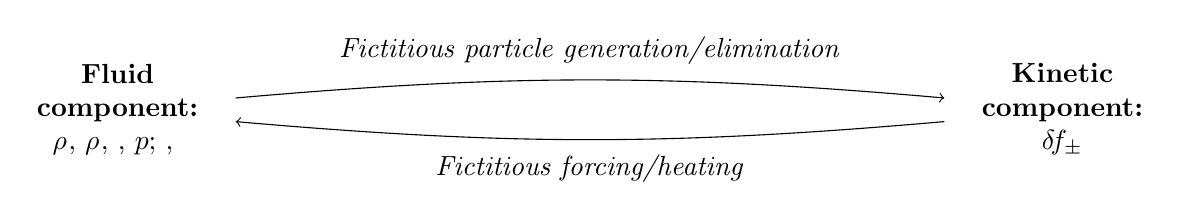
\begin{tikzpicture}[align = center, node distance = 4cm, auto]
            \node (1) at (0,  0) {\bf Fluid    \\  \bf component:  \\  $\rho_{\rmM}$, $\rho_{\rmC}$, $\bfp$, $p$; $\bfE$, $\bfB$};
            \node (2) at (12, 0) {\bf Kinetic  \\  \bf component:  \\  $\delta\!f_{\pm}$};
            
            \draw[->] (1.5, 0.15) to [out = 5, in = 175] (10.5, 0.15);
            \node at (6, 0.75) {\emph{Fictitious particle generation/elimination}};
            \draw[->] (10.5, - 0.15) to [out = 185, in = -5] (1.5, - 0.15);
            \node at (6, - 0.75) {\emph{Fictitious forcing/heating}};
        \end{tikzpicture}
        \caption{Illustration of the coupling between the fluid and kinetic components of a fully coupled $\delta\!f$ decomposition.}
        \label{fig:delta f coupling}
    \end{figure}
    
    Some classical models derived from $\delta\!f$ decompositions reduce this by ignoring the effects of the kinetic component on the fluid component, thus solving a set of MHD equations for the thermalized background, and observing how the corrections evolve ``on top of it'. This is done in many classical gyrokinetic models, including those in \cite{Parker_Lee_1993, Dimits_Lee_1993}. These models however naturally lose validity over time, as the kinetic effects can not affect the dynamics of the thermalized background, as is known to be so prominently the case in tokamak plasmas.
    
    While it is worth remembering that $\bfj^{(0)}$ does \emph{not} formally equal the current, $\bfj$, we shall henceforth drop the superscript $*^{(0)}$ on $\bfj^{(0)}$, i.e. we shall write as $\bfj^{(0)}$ as $\bfj$.
